% DO NOT COMPILE THIS FILE DIRECTLY!
% This is included by the other .tex files.

\begin{frame}[t,plain]
\titlepage
\end{frame}

\section{MISP ZeroMQ}
\begin{frame}
\frametitle{MISP ZeroMQ}
    MISP includes a flexible publish-subscribe model to allow real-time integration of the MISP activities:
    \begin{itemize}
        \item Event publication
        \item Attribute creation or removal
        \item Sighting
        \item User login
    \end{itemize}
    \begin{center}
        $\rightarrow$ Operates at global level in MISP
    \end{center}
\end{frame}

\begin{frame}
    \frametitle{MISP ZeroMQ}
MISP ZeroMQ functionality can be used for various model of integration or to extend MISP functionalities:
    \begin{itemize}
        \item Real-time search of indicators into a SIEM\footnote{Security Information \& Event Management}
        \item Dashboard activities
        \item Logging mechanisms
        \item Continuous indexing
        \item Custom software or scripting
    \end{itemize}
\end{frame}

\section{MISP-Dashboard: An introduction}
\begin{frame}
    \frametitle{MISP-Dashboard - Realtime activities and threat intelligence}
    \vspace{-10px}
    \begin{center}
        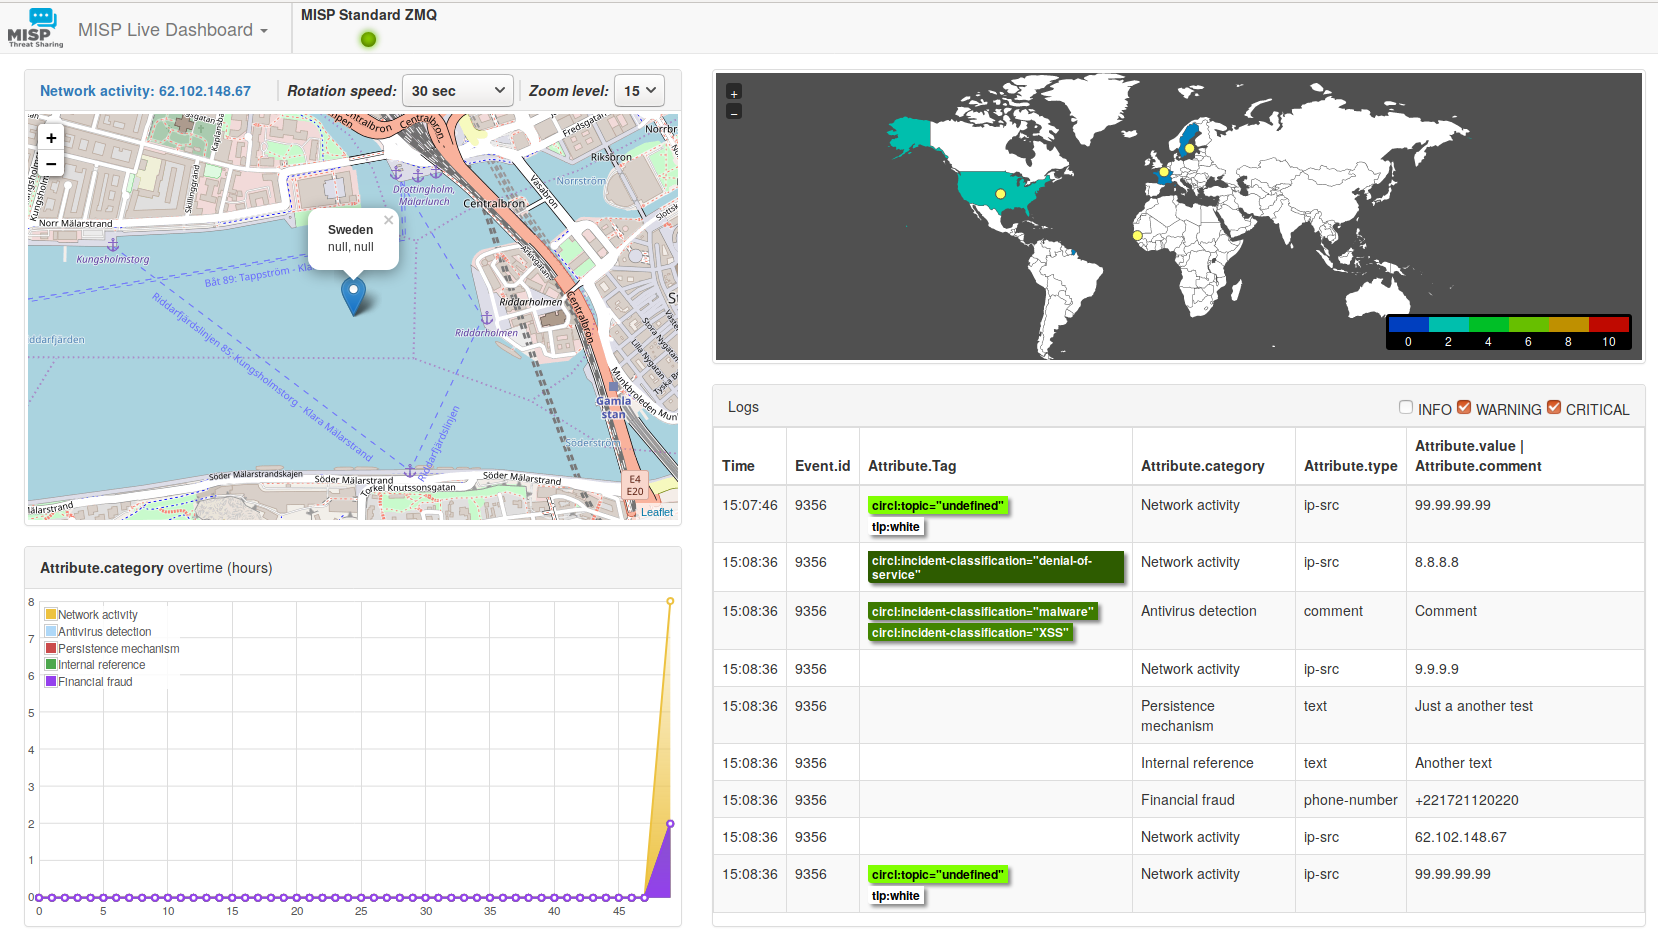
\includegraphics[width=1.00\linewidth]{images/dashboard-live.png}
    \end{center}
\end{frame}

\begin{frame}
\frametitle{MISP-Dashboard - Features}
    \vskip -0.5em
    \begin{center}
        \centering
        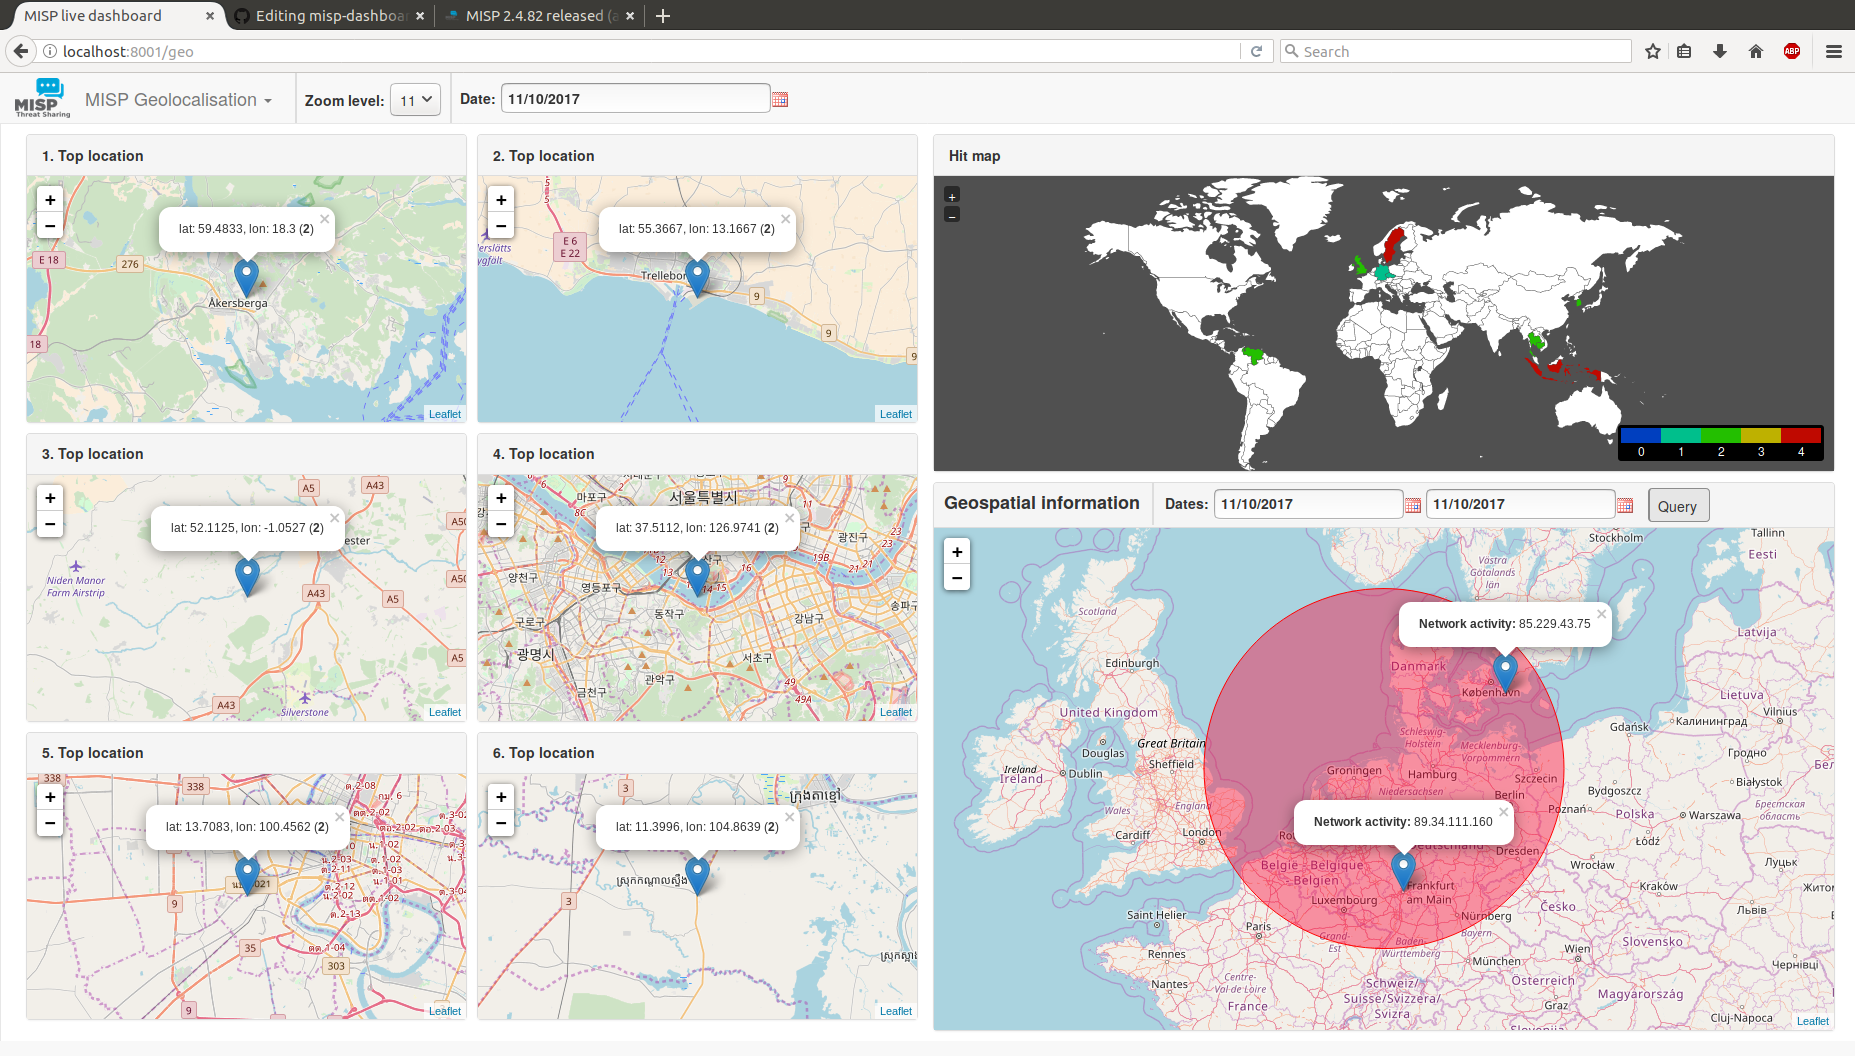
\includegraphics[scale=0.08]{images/dashboard-geo.png}
        $\;$
        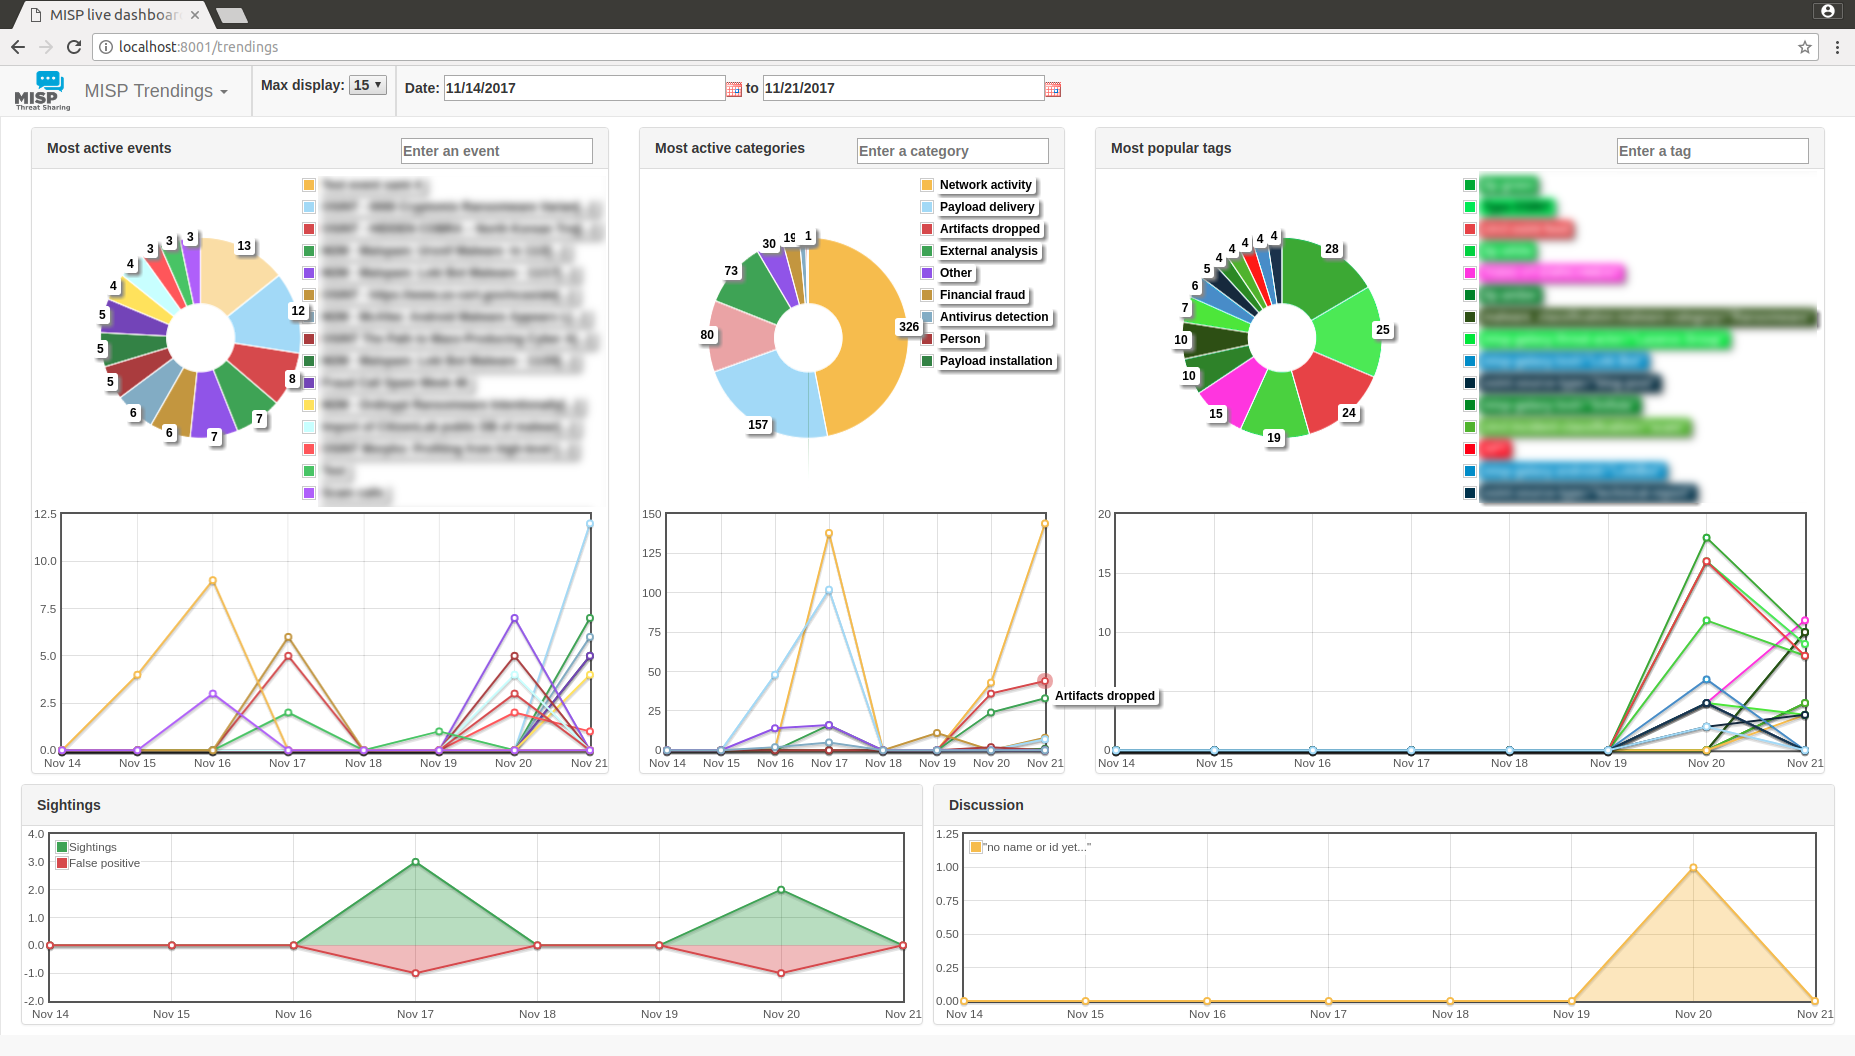
\includegraphics[scale=0.08]{images/dashboard-trendings.png}
    \end{center}
    \vskip -0.9em
    \begin{itemize}
        \item Subscribe to multiple \textbf{ZMQ} MISP instances
        \item Provides historical geolocalised information
        \item Present an experimental \textbf{Gamification of the platform}
        \item Shows when and how MISP is used
        \item Provides real time information showing current threats and activity
    \end{itemize}
\end{frame}

\section{MISP-Dashboard: Architecture and development}
\lstset{style=bash}
\begin{frame}[fragile]
\frametitle{Setting up the dashboard}
\begin{enumerate}
    \item Be sure to have a running redis server: e.g.
        \begin{itemize}
            \item \texttt{redis-server -p 6250}
        \end{itemize}
    \item Update your configuration in \texttt{config.cfg}
    \item Activate your virtualenv:
        \begin{itemize}
            \item \texttt{. ./DASHENV/bin/activate}
        \end{itemize}
    \item Listen to the MISP feed by starting the zmq\_subscriber:
        \begin{itemize}
            \item \texttt{./zmq\_subscriber.py}
        \end{itemize}
    \item Start the dispatcher to process received messages:
        \begin{itemize}
            \item \texttt{./zmq\_dispatcher.py}
        \end{itemize}
    \item Start the Flask server:
        \begin{itemize}
            \item \texttt{./server.py}
        \end{itemize}
    \item Access the interface at \url{http://localhost:8001/}
\end{enumerate}
\end{frame}

\begin{frame}
\textbf{\large MISP-Dashboard architecture}\\

\begin{center}
    \vskip -1.7em
    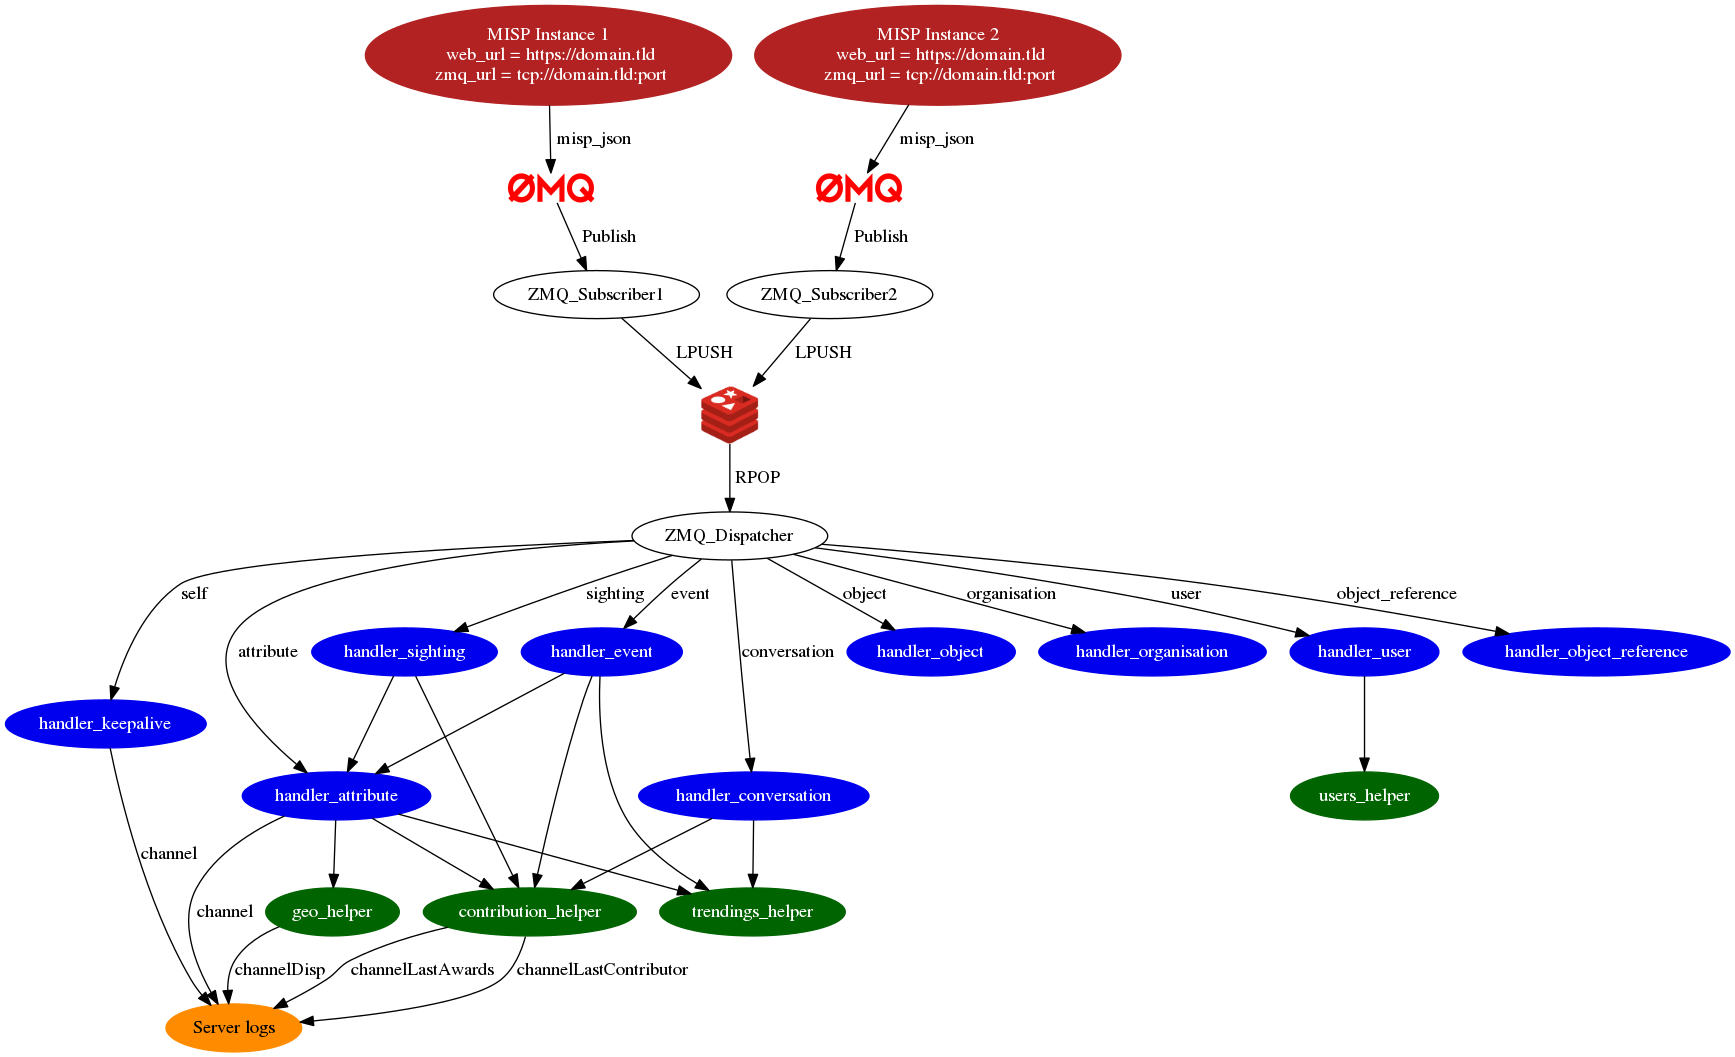
\includegraphics[scale=0.195]{images/messagepassing.png}
\end{center}
\end{frame}


\lstset{style=code,language=python}
\lstset{basicstyle=\fontsize{7}{9}\ttfamily}
\begin{frame}[fragile]
    \frametitle{Writing your handler}
    \begin{lstlisting}
# Register your handler
dico_action = {
        "misp_json":                  handler_dispatcher,
        "misp_json_event":            handler_event,
        "misp_json_self":             handler_keepalive,
        "misp_json_attribute":        handler_attribute,
        "misp_json_object":           handler_object,
        "misp_json_sighting":         YOUR_CUSTOM_SIGHTINGS_HANDLER,
        "misp_json_organisation":     handler_log,
        "misp_json_user":             handler_user,
        "misp_json_conversation":     handler_conversation,
        "misp_json_object_reference": handler_log,
}
    \end{lstlisting}
\end{frame}

\begin{frame}[fragile]
    \begin{lstlisting}
# Implement your handler

# e.g. user handler
def handler_user(zmq_name, jsondata):
    # json action performed by the user
    action = jsondata['action']
    # user json data
    json_user = jsondata['User']
    # organisation json data
    json_org = jsondata['Organisation']
    # organisation name
    org = json_org['name']
    # only consider user login
    if action == 'login':
        timestamp = time.time()
        # users_helper is a class to interact with the DB
        users_helper.add_user_login(timestamp, org)
    \end{lstlisting}
\end{frame}

\begin{frame}
        \frametitle{Recent changes in the misp-dashboard}
        \begin{itemize}
                \item MISP authentication can now be used in the misp-dashboard
                \item Improved TLS/SSL support in the default misp-dashboard
                \item Self-test tool to debug and test ZMQ connectivity
        \end{itemize}
\end{frame}

\begin{frame}
    \frametitle{Future development}
    \begin{itemize}
        \item[] 
\includegraphics[width=20px]{images/icons/joystick.png} \; Optimizing contribution scoring and model to encourage sharing and contributions enrichment
        \item[] 
\includegraphics[width=20px]{images/icons/globe.png} \; Increasing geolocation coverage
        \item[] 
\includegraphics[width=20px]{images/icons/zoom.png} \; Global filtering capabilities
            \begin{itemize}
                \item[] \quad - Geolocation: Showing wanted attribute or only on specific region
                \item[] \quad - Trendings: Showing only specified taxonomies
            \end{itemize}
        \item[] 
\includegraphics[width=20px]{images/icons/MISP.png} \; Tighter integration with MISP
            \begin{itemize}
                \item[] \quad - Present in MISP by default
                \item[] \quad - ACL enabled version
            \end{itemize}
    \end{itemize}
\end{frame}

\begin{frame}
   \frametitle{Conclusion}
MISP-Dashboard can provides realtime information to support security teams, CSIRTs or SOC showing current threats and activity by providing:
    \begin{itemize}
        \item Historical geolocalised information
        \item Geospatial information from specific regions
        \item The most active events, categories, tags, attributes, ...
    \end{itemize}

\vskip 0.5em
It also propose a prototype of gamification of the platform providing incentive to share and contribute to the community
\end{frame}


